%%%%%%%%%%%%%%%%%%%%%%%%%%%%%%%%%%%%%%%%%%%%%%%%%%%%%%%%%%%%%%%%%%%%%%
%%                     Or
%%%%%%%%%%%%%%%%%%%%%%%%%%%%%%%%%%%%%%%%%%%%%%%%%%%%%%%%%%%%%%%%%%%%%%
%\color{blue}
\subsection{Glyph: \glyph{Or}}\label{sec:or}

The glyph \glyph{or} is used to denote that any of the \glyph{EPNs} linked as input is sufficient to produce the output.  

\begin{glyphDescription}
 \glyphSboTerm SBO:0000174 ! or.
 \glyphOrigin More than one \glyph{EPN} (section~\ref{sec:EPNs}) or \glyph{logical operator} (section~\ref{sec:logic}).
 \glyphTarget  One modulation (section~\ref{sec:modulation}), stimulation (section~\ref{sec:stimulation}), catalysis (section~\ref{sec:catalysis}), inhibition (section~\ref{sec:inhibition}) or necessary stimulation (section~\ref{sec:necessary_stim}) arc.
 \glyphNode \glyph{Or} is represented by a circle carrying the word ``OR''.
 \end{glyphDescription}

\begin{figure}[H]
  \centering
  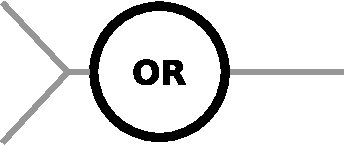
\includegraphics[scale = 0.5]{images/or}
  \caption{The \PD glyph for \glyph{or}. Only two inputs are represented, but more would be allowed.}
  \label{fig:or}
\end{figure}


